% \title{Desktop Calendar (fits CD jewel case)}

%%% The calendars are printed 2-up to fit CD jewel cases,
%%% or 4-up to fit 3" floppy disk jewel cases. OR, now a
%%% full-blown "giant" version that prints full-page!
%%%
%%% Localisation possible with languages supported by
%%% babel/translator/datetime2.
%%% Tested with british, spanish, french, ngerman,
%%% italian, portuges, polish, croatian, greek, bahasai,
%%% bahasam.
%%%
%%% bahasai (Indonesian) works with the following new or
%%% modified files in this project:
%%% - translator-language-mappings.tex
%%% - translator-months-dictionary-Indonesian.dict
%%% - datetime2-bahasai.ldf
%%%
%%% bahasam (Bahasa Malaysia) works with the following new or
%%% modified files in this project:
%%% - translator-language-mappings.tex
%%% - translator-months-dictionary-Malaysian.dict
%%% - datetime2-bahasam.ldf
%%%
%%% (Use lualatex for french. If using pdflatex for greek,
%%% Remember to load LGR,T1 for fontenc.)
\documentclass[12pt,british]{cdcalendar}
%%% Use the sundayweek option for weeks to start on Sundays.
% \documentclass[12pt,british,sundayweek]{cdcalendar}
%% If using pdfLaTeX %%%%%%%%%%
\usepackage[utf8]{inputenc}
\usepackage[T1]{fontenc}

% Using Gentium and Open Sans
\usepackage{gentium}
\usepackage[defaultsans,osfigures,scale=0.94]{opensans}
%% End pdfLaTeX-related font settings %%%%%%%%


% %% Compile with luaLaTeX if using fontspec
% \usepackage{fontspec}
% \setmainfont{Gentium}
% \setsansfont[BoldItalicFont=Fira Sans Italic,BoldFont=Fira Sans]{Fira Sans Light}
% %% End luaLaTeX-related font settings %%%%%%%%


\usepackage{graphicx}
\usepackage{wallpaper}
\usepackage{fontawesome}
\graphicspath{{img/}}

\tikzset{blue icon/.style={text=SkyBlue,font=\Large}}
\tikzset{orange icon/.style={text=orange!60,font=\Large}}

\begin{document}

%%%%%%
% Cover
%%%%%%
\coverBgColor{RoyalBlue!40!black}
\coverImage{LuncheonoftheBoatingParty}
\coverTitle[font=\fontsize{30pt}{32pt}\sffamily\bfseries,text=white,text width=\linewidth,align=flush right]{Coventry City Council 2015/16 School Year}

\makeCover

%%%% Remove this page if you don't need it --
%%%% just to show the actual output
{\centering
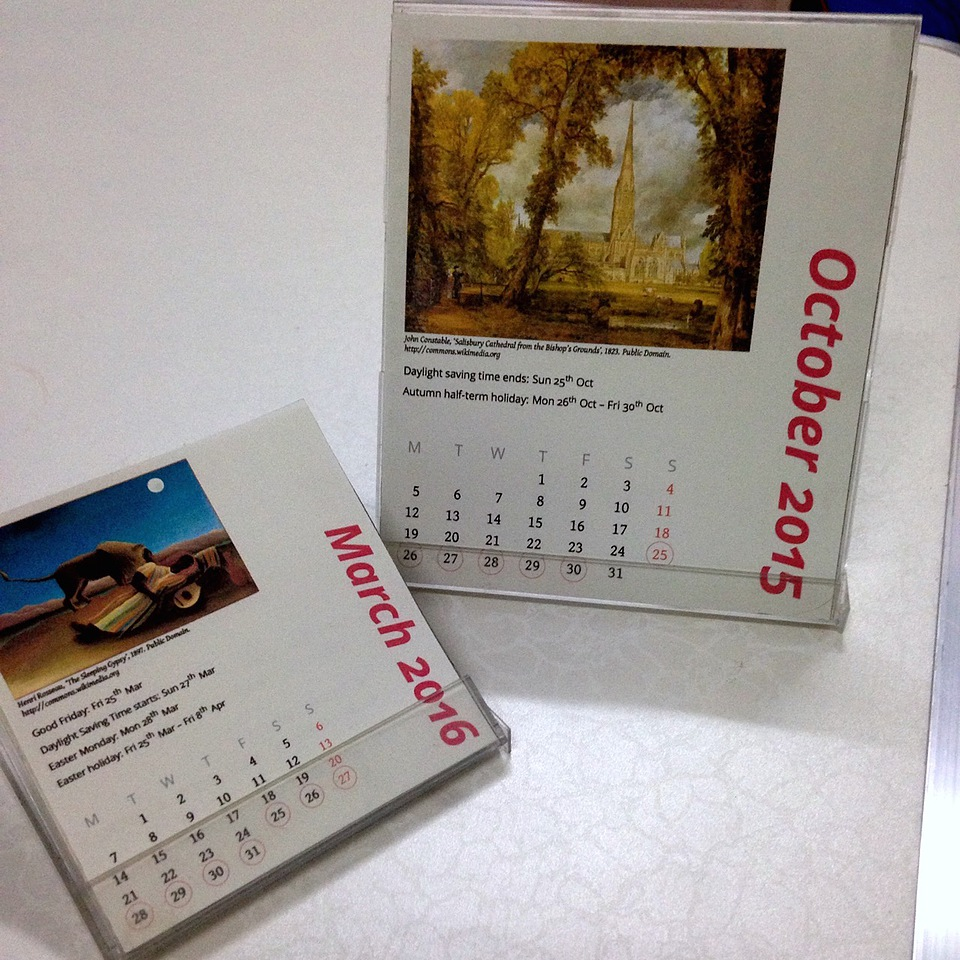
\includegraphics[width=\textwidth]{actual}
\par}

Here are the actual printed calendars. The smaller calendar (9cm $\times$ 9.5cm) fits floppy disk jewel cases; while the bigger one (11.7cm $\times$ 13.65cm) fits CD jewel cases.

\clearpage
%%%%


%%%%%%
% Some settings for the monthly calendars
%%%%%%
\dayHeadingStyle{font=\sffamily\color{gray!90}}
\sundayColor{red}
\monthTitleStyle{font={\fontsize{42pt}{44pt}\bfseries\sffamily\itshape\selectfont}, red!50!RedViolet}
\eventStyle{\scriptsize\sffamily}

% Remove this line if you feel the background pattern is too annoying
\TileWallPaper{.5\paperwidth}{.5\paperheight}{ricepaper_v3}

% You may find the gap between illustrations and events too wide
% Use this length to lessen it
\setlength{\lessIllusSkip}{1ex}


%%%%%%
% September 2015
%%%%%%
\illustration[Vincent van Gogh, `The Starry Night', 1889. Public Domain. \url{http://commons.wikimedia.org}]{8.5cm}{StarryNight}

\begin{monthCalendar}{2015}{09}

%%% events must be given AFTER \begin{monthCalendar}
%%% Currently you must give events on the same page
%%% as the monthly calendar.

%% This is an one-day event
\event[mark style=orange icon, marker=\faBook]{2015-09-02}{}{Autumn school term starts}

\end{monthCalendar}

\clearpage


%%%%%%
% Oct 2015
%%%%%%
\illustration[John Constable, `Salisbury Cathedral from the Bishop's Grounds', 1823. Public Domain. \url{http://commons.wikimedia.org}]{8.5cm}{SalisburyCathedral}

\begin{monthCalendar}{2015}{10}

\event[mark style=blue icon, marker=\faClockO]{2015-10-25}{}{Daylight saving time ends}

%% This is a 5-day event starting Oct 26th
\event{2015-10-26}{5}{Autumn half-term holiday}

%% You could also write
%\event{2015-10-26}{2015-10-30}{Autumn half-term holiday}

\end{monthCalendar}

\clearpage

%%%%%%
% Nov 2015
%%%%%%
\illustration[Jin Nong, `Flower', 1754. Public Domain. \url{http://commons.wikimedia.org}]{8.5cm}{Flower_JinNong}

\begin{monthCalendar}{2015}{11}

\end{monthCalendar}

\clearpage


%%%%%%
% Dec 2015
%%%%%%
\illustration[Hendrick Avercamp, `Winter Landscape with Ice Skaters', c.~1608. Public Domain. \url{http://commons.wikimedia.org}]{8.5cm}{WinterLandscape}

\begin{monthCalendar}{2015}{12}

\event{2015-12-18}{}{Last day of Autumn term}

\event{2015-12-25}{}{Christmas Day}

\event{2015-12-28}{}{Boxing Day (substitute)}

\end{monthCalendar}

\clearpage

%%%%%%
% January 2016
%%%%%%
\illustration[Auguste Renoir, `Oarsmen at Chatou', 1879. Open Access. \url{https://images.nga.gov}]%
{8.5cm}{A17050}

\begin{monthCalendar}{2016}{01}

\event{2016-01-01}{}{New Year's Day}

\event[mark style=orange icon, marker=\faBook]{2016-01-04}{}{Spring term starts}

\end{monthCalendar}

\clearpage

%%%%%%
% February 2016
%%%%%%
\illustration[Cariani, `Concert', c.~1518--1520. Open Access. \url{https://images.nga.gov}]%
{8.5cm}{A10623}

\begin{monthCalendar}{2016}{02}

%% This is a 5-day event starting on Feb 15
\event{2016-02-15}{5}{Spring half-term holiday}

\end{monthCalendar}

\clearpage

%%%%%%
% March 2016
%%%%%%
\illustration[Henri Rosseau, `The Sleeping Gypsy', 1897. Public Domain. \url{http://commons.wikimedia.org}]{8.5cm}{SleepingGypsy}

\begin{monthCalendar}{2016}{03}

\event{2016-03-25}{}{Good Friday}

\event[mark style=blue icon, marker=\faClockO]{2016-03-27}{}{Daylight Saving Time starts}

\event{2016-03-28}{}{Easter Monday}


%% Note if a multi-day event extends to the next month,
%% you'll have to list it again in the next month.
\event{2016-03-25}{2016-04-08}{Easter holiday}

\end{monthCalendar}

\clearpage


%%%%%%
% April 2016
%%%%%%
\illustration[Katsushika Hokusai, `The Great Wave of Kanagawa', 1823--1829. Public Domain. \url{http://commons.wikimedia.org}]{8.5cm}{Tsunami}

\begin{monthCalendar}{2016}{04}

\event{2016-03-25}{2016-04-08}{Easter holiday}

\end{monthCalendar}

\clearpage

%%%%%%
% May 2016
%%%%%%
\illustration[John Everett Millais, `Ophelia', circa 1851. Public Domain. \url{http://commons.wikimedia.org}]{8.5cm}{Ophelia}

\begin{monthCalendar}{2016}{05}

\event[mark style=blue icon, marker=\faBank]{2016-05-02}{}{Early May bank holiday}

\event[mark style=blue icon, marker=\faBank]{2016-05-30}{}{Spring Bank Holiday}

\event{2016-05-30}{5}{Summer half-term holiday}

\end{monthCalendar}

\clearpage

%%%%%%
% June 2015
%%%%%%
% {\huge\color{BurntOrange} Deep summer is when laziness finds respectability.\par}
% {\raggedleft -- Sam Keen\par}
\illustration[J.M.W.~Turner, `The Fighting Temeraire tugged to her last berth to be broken up', 1839. Public Domain. \url{http://commons.wikimedia.org}]{8.5cm}{FightingTemeraire}

\begin{monthCalendar}{2016}{06}

\event{2016-05-30}{5}{Summer half-term holiday}

\end{monthCalendar}

\clearpage

%%%%%%
% July 2016
%%%%%%
\illustration[Édouard Manet, `A Bar at the Folies-Bergère', 1881 -- 1882. Public Domain. \url{http://commons.wikimedia.org}]{8.5cm}{BarAtTheFoliesBergere}

\begin{monthCalendar}{2016}{07}

\event{2016-07-21}{}{Summer holiday begins}
\end{monthCalendar}

\clearpage

%%%%%%
% August 2016
%%%%%%
\illustration[Georges Seurat, `A Sunday Afternoon on the Island of La Grande Jatte', 1884 -- 1886. Public Domain. \url{http://commons.wikimedia.org}]{8.5cm}{SundayOnLaGrandeJatte}

\begin{monthCalendar}{2016}{08}

\event[mark style=blue icon, marker=\faBank]{2016-08-29}{}{Summer bank holiday}
\event[mark style=blue icon, marker=\faBank]{2016-09-06}{}{New school year begins}

\end{monthCalendar}

\clearpage

\end{document}
